\section{System overview}
\paragraph{}
Our team has 5 robots comprised of 2 sizes; 3 with 57 cm in height, and 2 with of 47 cm in height as shown in Fig 1. Each robot is composed of mechanical hardware, sensors, and computing hardware. The structure of all robots is made of aluminum alloy sheet. Each robot uses 20 servo-motors to control mechanical joints: 6 DOF in each leg, 3 DOF per arm and 2 DOF on head.Our team has 3 robots. Each robot is composed of mechanical hardware, sensors, and computing hardware. The structure of all robots is made of aluminum alloy sheet metal. Each robot uses 20 servo-motors (details are provided in the robot specification sheet).
\begin{figure}[H]
	\centering
	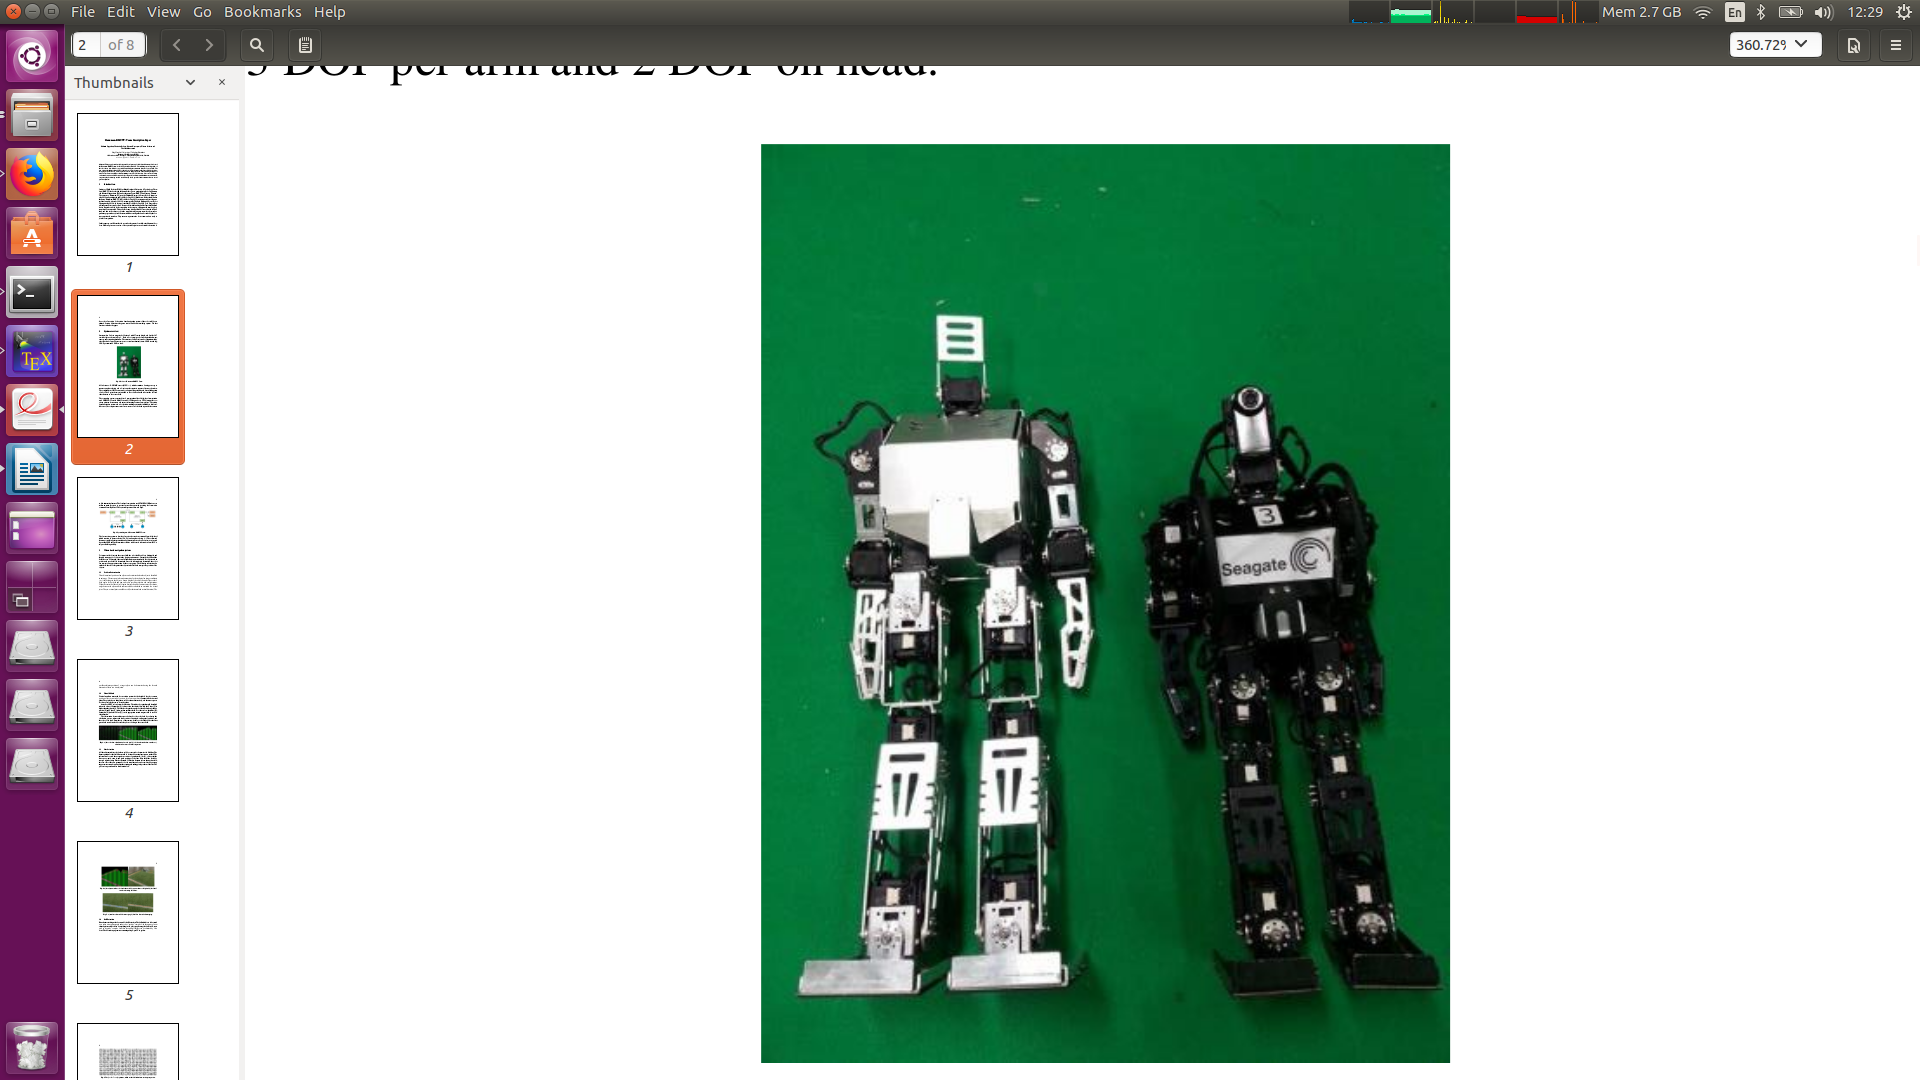
\includegraphics[width=\textwidth,trim={15cm 0cm 5cm 5cm},clip]{image/humanoid.png}
	\caption{Robots of Hanuman-KMUTT Team}
	\label{fig:humanoid}
\end{figure}
All robots use 6 DOF IMU sensor (MPU- 6500 ) which contains a 3-axis gyroscope to measure angular velocity and a 3-axis accelerometer to measure linear acceleration. The combination of IMU sensor used to adapt walking stability and detect falling state of robot. The Logitech camera installed on the robot head used to detect the ball and other features on the soccer field. The computing system separated into 2 computational level: high-level computation used ODROID-C1+ with ARM Cortex-A5 (1.5Ghz quad core CPUs) computer to receives pictures from camera and extract interesting features from picture. The vision based navigation system and robot decision-making system also installed on this level. Moreover, the computer can control servo-motors on robot head to pan-tilt the camera3 to find interesting features. The low-level computation used STM32F411RE micro-controller as main processor to operate locomotion system by receiving the locomotion command from high-level. The system diagram as shown in \ref{fig:sysDiagram}
\begin{figure}[H]
	\centering
	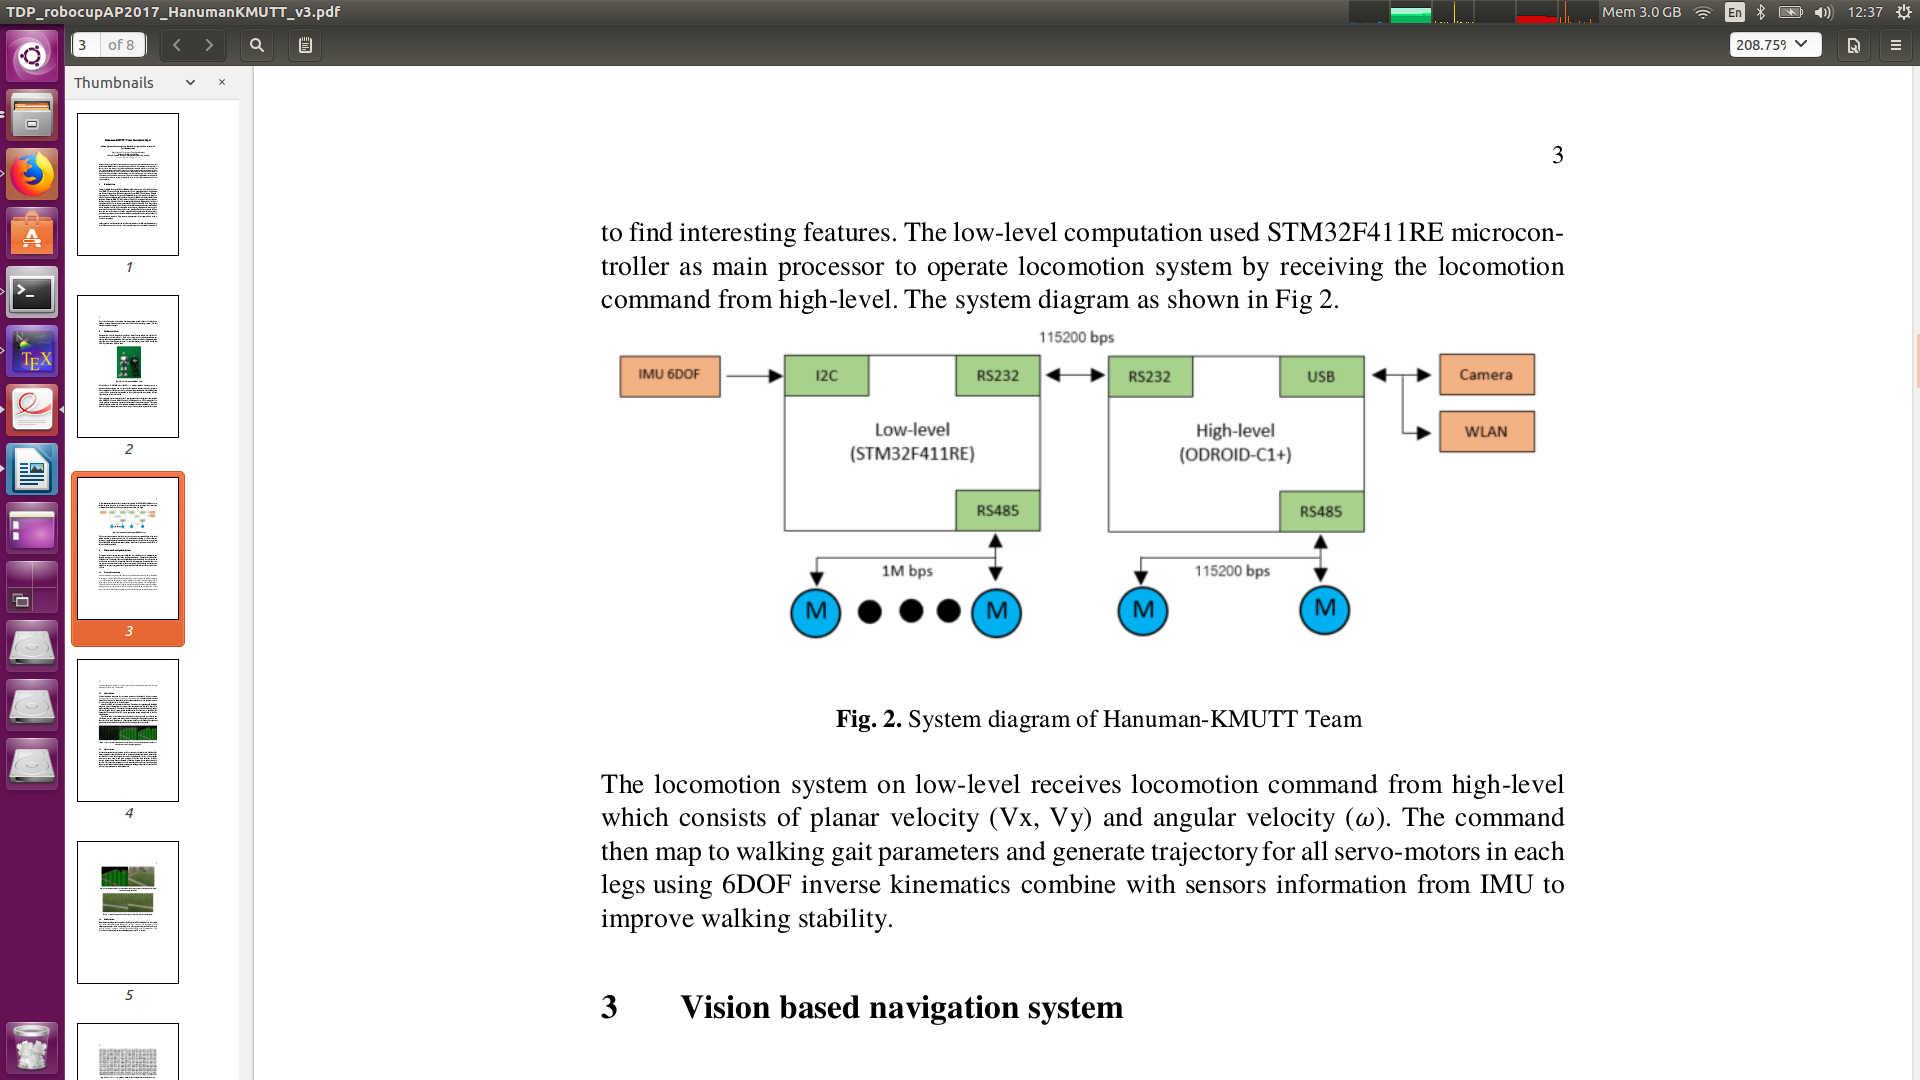
\includegraphics[width=\textwidth,trim={20cm 15cm 10cm 12.5cm},clip]{image/sysDiagram.png}
	\caption{System diagram of Hanuman-KMUTT Team}
	\label{fig:sysDiagram}
\end{figure}
The locomotion system on low-level receives locomotion command from high-level
which consists of planar velocity (Vx, Vy) and angular velocity (ω). The command
then map to walking gait parameters and generate trajectory for all servo-motors in each
legs using 6DOF inverse kinematics combine with sensors information from IMU to
improve walking stability.